\section{Analytic Treatment}

%% Main colours from thesis
\definecolor{PeelingPaper}{RGB}{5,135,137}
\definecolor{WoodenPlatforms}{RGB}{80,61,46}
\definecolor{Puzzle24000}{RGB}{213,75,26}
\definecolor{Escape}{RGB}{227,167,47}

\definecolor{Tropiteal}{RGB}{0,168,198}
\definecolor{TealDrop}{RGB}{64,192,203}
\definecolor{WhiteTrash}{RGB}{249,242,231}
\definecolor{AtomicBikini}{RGB}{174,226,57}
\definecolor{FeebleWeek}{RGB}{143,190,0}
\definecolor{ICantExpress}{RGB}{28,20,13}
\definecolor{Marty}{RGB}{250,42,0}
\definecolor{WeddedPassion}{RGB}{164,7,120}

% Colours from the beamer theme
\definecolor{mDarkBrown}{HTML}{604c38}
\definecolor{mDarkTeal}{HTML}{23373b}
\definecolor{mLightBrown}{HTML}{EB811B}
\definecolor{mLightGreen}{HTML}{14B03D}

% Colour definitions
%\colorlet{ColourBase}{PeelingPaper}
\colorlet{ColourBase}{mLightGreen}
%\colorlet{ColourHl1}{Puzzle24000}
\colorlet{ColourHl1}{mLightBrown}
%\colorlet{ColourHl2}{FeebleWeek}
\colorlet{ColourHl2}{PeelingPaper}
\colorlet{ColourHl3}{Escape}
\colorlet{ColourDark}{mDarkTeal}
\colorlet{ColourDark2}{mDarkBrown}


\usetikzlibrary{decorations}
\usetikzlibrary{decorations.markings,decorations.pathmorphing}
\usetikzlibrary{arrows.meta, bending}
\usetikzlibrary{shapes.geometric}

\colorlet{col1}{ColourHl1}
\colorlet{col2}{ColourBase}
\colorlet{col3}{ColourDark2}
\colorlet{col4}{ColourDark}

% Graph styles from my phd thesis
\tikzset{
  graph style/.style={
    baseline={([yshift=-.5ex]current bounding box.center)},
    node distance=1,
  },
  skeleton node/.style={
    black,fill,circle,inner sep=0pt,minimum size=3.5pt
  },
  skeleton bond/.style={
    draw,
  },
}

% Graph styles from previous presentations
\tikzset{
  inner/.style={
    fill=#1,
    circle,
    inner sep=0pt,
    minimum size=4
  },
  outer/.style={
    draw=#1,
    thick,
    circle,
    inner sep=0pt,
    minimum size=7,
  },
  outerouter/.style={
    draw=#1,
    thick,
    circle,
    inner sep=0pt,
    minimum size=10,
  },
  linestyle/.style={
    thick,
  },
  inner1/.style={
    inner=col1,
  },
  inner2/.style={
    inner=col2,
  },
  inner3/.style={
    inner=col3,
  },
  outer1/.style={
    outer=col1,
  },
  outer2/.style={
    outer=col2,
  },
  outer3/.style={
    outer=col3,
  },
  resum node/.style={
    %fill=ColourDark2,
    fill=ColourHl2,
    regular polygon,
    regular polygon sides=6,
    inner sep=0pt,
    minimum size=5pt
  },
  ->-/.style={decoration={
    markings,
    mark=at position #1 with {\arrow{Stealth[angle=45:6pt,flex,round]}}},
    postaction={decorate}
  },
  -<-/.style={decoration={
    markings,
    mark=at position #1 with {\arrow{Stealth[angle=45:6pt,round,flex,reversed]}}},
    postaction={decorate}
  }
}


% Bond styles from my phd thesis
\tikzset{
  bond default/.style={
    skeleton bond,
    line width=1.2pt,
  },
  bond 1/.style={
    bond default,
    ColourBase,
  },
  bond 2/.style={
    bond default,
    ColourHl1,
  },
  bond 3/.style={
    bond default,
    ColourHl2,
  },
  bond 4/.style={
    bond default,
    ColourDark2,
  },
}

% ------------------------------------------- %
% position function                           %
% http://tex.stackexchange.com/a/102266/39313 %
% ------------------------------------------- %

\makeatletter
\tikzset{
  position/.style args={#1 degrees from #2}{
    at=(#2.#1), anchor=#1+180, shift=(#1:\tikz@node@distance)
  }
}
\makeatother


\begin{frame}{Motivation}


  \IfFileExists{include/luscher_weisz_triviality.pdf}{%
    \begin{center}
      \includegraphics[page=1, trim={0 9.85cm 0 3cm}, clip, width=\textwidth]{include/luscher_weisz_triviality.pdf}
    \end{center}
  }{%
    \vfill
    \tikz \node[draw, ColourHl1, minimum height=.8\textheight] {%
      \begin{minipage}{\textwidth}
        \begin{center}\color{ColourHl1}%
          Lüscher \& Weisz: $\lambda \phi^4$ triviality
        \end{center}
      \end{minipage}};
    \vfill
  }

\end{frame}

\begin{frame}{The linked cluster expansion}

\nointerlineskip
\begin{tikzpicture}[overlay,remember picture]

  \coordinate (top left) at ([yshift=-1.04cm] current page.north west);
  \coordinate (top right) at ([yshift=-1.04cm] current page.north east);
  \coordinate (top) at ([yshift=-1.04cm] current page.north);
  \coordinate (bottom left) at (current page.south west);
  \coordinate (bottom right) at (current page.south east);
  \coordinate (bottom) at (current page.south);
  \coordinate (mid left) at ([yshift=-0.52cm] current page.west);
  \coordinate (mid right) at ([yshift=-0.52cm] current page.east);
  \coordinate (mid) at ([yshift=-0.52cm] current page.center);

  \fill [ColourHl1,  opacity=0.175] (top left) rectangle (mid right);
  \fill [ColourBase, opacity=0.175] (mid left) rectangle (bottom right);

  \draw [ColourDark] (mid left) -- (mid right);

  \node at ([shift={(.5cm, -.5cm)}] top left) [anchor=north west, scale=1.25] {%
    $\lambda \phi^4$ theory};

  \node at ([yshift=-.25cm] $ (top)!0.5!(mid) $) [anchor=center] {%
    \begin{minipage}{\textwidth}
      \[
        \int \prod \mathrm{d} \phi(x) \, \exp \bigg\{ -S_0[\phi]
          - \kappa \sum_{\langle x,y \rangle} \phi(x) \phi(y) \bigg\}
      \]
    \end{minipage}};


  \node at ([shift={(.5cm, -.5cm)}] mid left) [anchor=north west, scale=1.25] {%
    The effective theory};

  \node at ([yshift=-.25cm] $ (mid)!0.5!(bottom) $) [anchor=center] {%
    \begin{minipage}{\textwidth}
      \[
      \int \prod \mathrm{d} L(x) \, \det Q^{\mathrm{stat}} \exp \bigg\{- \lambda \sum_{\langle x, y \rangle} L(x) L^*(y) + ... \bigg\}
      \]
    \end{minipage}};
  
\end{tikzpicture}
  
\end{frame}

\begin{frame}{The two step embedding procedure}
  \begin{tikzpicture}[overlay,remember picture]

    \node[anchor=north west] (eff-title) at ([shift={(1cm, -1.5cm)}] current page.north west) {%
      Effective theory terms};

    \node[below=0.2cm of eff-title] (eff-graphs) {%
      \includegraphics{effective_theory_graph1} \hspace{.75cm}
      \includegraphics{effective_theory_graph2}};

    \node[below=2.75cm of eff-graphs] (skel) {%
      \includegraphics{graph_skel}};
    \node[below=.2cm of skel] (skel-title) {%
      LCE skeleton graph};

    \draw[
      thick, ColourDark, -{Stealth[round]},
      postaction={decorate,decoration={text along path, text align=center, text={|\footnotesize|embedding}, raise=.75ex}},
    ] ([yshift=-.2cm] eff-graphs.south) -- ([yshift=.2cm] skel.north);

    \node [right=4.5cm of eff-graphs, yshift=.75cm] (emb1) {%
      \includegraphics{graph_emb1}};

    \node [below=.5cm of emb1] (emb2) {%
      \includegraphics{graph_emb2}};

    \node [below=.5cm of emb2] (emb3) {%
      \includegraphics{graph_emb3}};

    \node [below=.5cm of emb3] (emb4) {%
      \includegraphics{graph_emb4}};

    \draw[
      thick, ColourDark, -{Stealth[round]},
      postaction={
        decorate,
        decoration={
          text along path, text color=ColourHl1,
          text align={right, right indent=.9cm},
          text={|\footnotesize|results in}, raise=.75ex
        },
      },
    ] ([xshift=.5cm] skel.east) ..
      controls +(3cm, 0) and +(-3cm, 0) ..
      ([xshift=-.5cm] emb1.west);
  \end{tikzpicture}
\end{frame}

\begin{frame}[plain]{}
  \begin{tikzpicture}[overlay,remember picture]
    \node[anchor=center] at (current page.center) {\includegraphics[scale=1.6]{graphmatrix}};
  \end{tikzpicture}
\end{frame}

\begin{frame}{Analytical resummation}

  Look to the \alert{resummed linked cluster expansion} for inspiration

  \vspace{1em}

  \begin{center}
    \includegraphics[width=\textwidth]{graph_resummation}
  \end{center}

  \vspace{.5em}

  We can implement the same resummation on the level of the effective theory
  itself, incorporating \alert{long range effects}

  \[
    
\begin{tikzpicture}[graph style]
  \node[inner2] (n1) {};
  \node[outer1] (n1o) at (n1) {};
  \node[inner2] (n2) [position=60 degrees from n1] {};
  \node[outer1] (n2o) at (n2) {}
    edge[bond 1, bend left=45]  (n1o)
    edge[bond 2, bend right=45] (n1o);
  \node[resum node] (n3) [position=300 degrees from n2] {}
    edge[bond 2] (n2o);
\end{tikzpicture}
\:=\:

\begin{tikzpicture}[graph style]
  \node[inner2] (n1) {};
  \node[outer1] (n1o) at (n1) {};
  \node[inner2] (n2) [position=60 degrees from n1] {};
  \node[outer1] (n2o) at (n2) {}
    edge[bond 1, bend left=45]  (n1o)
    edge[bond 2, bend right=45] (n1o);
  \node[inner1] (n3) [position=300 degrees from n2] {}
    edge[bond 2] (n2o);
\end{tikzpicture}
\:+\:

\begin{tikzpicture}[graph style]
  \node[inner2] (n1) {};
  \node[outer1] (n1o) at (n1) {};
  \node[inner2] (n2) [position=60 degrees from n1] {};
  \node[outer1] (n2o) at (n2) {}
    edge[bond 1, bend left=45]  (n1o)
    edge[bond 2, bend right=45] (n1o);
  \node[inner1] (n3) [position=300 degrees from n2] {}
    edge[bond 2] (n2o);
  \node[inner1] (n4) [position=60 degrees from n3] {}
    edge[bond 2] (n3);
\end{tikzpicture}
\:+\:
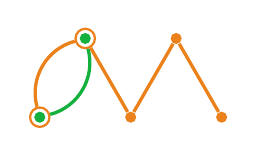
\begin{tikzpicture}[graph style]
  \node[inner2] (n1) {};
  \node[outer1] (n1o) at (n1) {};
  \node[inner2] (n2) [position=60 degrees from n1] {};
  \node[outer1] (n2o) at (n2) {}
    edge[bond 1, bend left=45]  (n1o)
    edge[bond 2, bend right=45] (n1o);
  \node[inner1] (n3) [position=300 degrees from n2] {}
    edge[bond 2] (n2o);
  \node[inner1] (n4) [position=60 degrees from n3] {}
    edge[bond 2] (n3);
  \node[inner1] (n5) [position=300 degrees from n4] {}
    edge[bond 2] (n4);
\end{tikzpicture}
\:\dots

\]
  
\end{frame}

\begin{frame}{Results: Convergence}

  \begin{center}
    \includegraphics[width=\textwidth]{nb_of_h2_resummed_comparison}
  \end{center}
  
\end{frame}

\begin{frame}{Results: Towards lighter quarks}

  \vspace{.5cm}

  \begin{center}\hspace*{-1cm}
    \includegraphics[width=.9\textwidth]{nb_of_mpi_a01_r}
  \end{center}
  
\end{frame}

\begin{frame}{Results: The equation of state}

  \vspace{.25cm}
  \begin{center}
    \includegraphics[width=\textwidth]{nb_of_press_scaled}
  \end{center}
  
\end{frame}

\begin{frame}{Other applications: SU($N$)}

  \begin{center}
    \includegraphics[width=.7\textwidth]{nb_of_mu_diff_nc}
  \end{center}

  \vspace*{-.5cm}

  \begin{overprint}
    \onslide<1>
      The procedure is easily extendable to \alert{other gauge groups}, escpecially
      other SU($N$)
    \onslide<2>
      As $N$ increases the \alert{gauge sector} will once again be
      \alert{important} and start competing with the fermionic contribution
  \end{overprint}

\end{frame}
